\section{实验}

本章在同一冻结骨干和评价脚本下比较QDPT、静态Prompt、实例条件Prompt与LoRA，并分析Prompt输入位置、训练效率与随机种子稳定性。

\subsection{实验设置}

\subsubsection{数据集}

视觉问答要求模型根据图像和自然语言问题生成答案\cite{Agrawal2015VQAVQ}。PathVQA\cite{He2020PathVQA3Q}是主要开发数据集。结构选择在官方Validation划分上完成，Test划分仅用于最终配置的评估。本文同时报告Overall、Yes/No和Free-form准确率，以区分封闭式判断与开放式生成。

SLAKE\cite{Liu2021SlakeAS}用于检查同一结构在另一数据集上的表现。两个公开数据集使用相同的QDPT结构配置。除Overall外，实验还统计CLOSED与OPEN、KVQA与VQA，以及英文和中文问题。

自建电力电气数据集由本实验室采购的电力设备图像及目标检测标注整理而成。训练集包含20,015张图像，并借助Gemma 3 27B IT将检测标签、类别、目标数量和场景信息转换为36,700条多模态指令，任务包括设备与部件识别、缺陷与异常判断。固定测试集包含972张训练集之外的图像，每张图像对应一道经过人工核对的选择题。其中18个样本因图像文件关联缺失被排除，所有方法均在相同的954个有效样本上计算准确率。该数据集不公开。

\subsubsection{比较方法}

所有方法使用同一Qwen3-VL骨干\cite{Bai2025Qwen3VLTR}、图像预处理和答案评估脚本。Static LLM Prompt、Static Visual Prompt与Dual Static Prompt分别在语言侧、视觉侧或两侧加入样本共享的连续Prompt\cite{lester2021power,jia2022visual}。CoCoOp-style是CoCoOp\cite{Zhou2022ConditionalPL}在生成式MLLM上的近似复现：保留图像条件Meta-Net与共享连续上下文，用Merger输出的图像Token均值生成条件偏置，并将其加到语言Prompt上。Full-Attention LoRA-r8\cite{Hu2022LoRA}在视觉编码器和语言模型的全部注意力层加入秩为8的低秩更新，作为权重空间适配参照。GRASP\cite{Sun2026GRASPGR}没有可用的官方代码，独立实现及核验过程移至附录\ref{sec:grasp-appendix}，不参与主表排序。

\subsubsection{训练与评价协议}

实验使用单张NVIDIA GeForce RTX 5090，软件环境为PyTorch 2.8.0、torchvision 0.23.0和Transformers 5.0.0；PyTorch与torchvision均为CUDA 12.8构建，驱动支持CUDA 13.0。所有方法使用BF16精度并冻结原始骨干参数，仅优化新增适配参数。输入采用Qwen3-VL原始AutoProcessor的动态分辨率策略，各方法均未额外指定固定图像分辨率或视觉Token上限，文本序列最大长度为2048。

QDPT使用AdamW，$\beta_1=0.9$、$\beta_2=0.999$、$\epsilon=10^{-8}$，所有参数组的权重衰减为0。学习率在前3\%训练步内线性预热，随后线性衰减；梯度范数裁剪阈值为1.0，不使用梯度检查点。训练共3个epoch，单卡微批量为2，梯度累积16步，有效batch size为32。20个静态语言Prompt $P^t$与10个文本Anchor $A^t$的学习率为0.3。18个静态视觉Prompt分为两组：前8个使用$3\times10^{-5}$，其余10个使用$10^{-4}$；问题池化、视觉投影、跨注意力与输出映射均使用$10^{-4}$。

Full-Attention LoRA采用$r=8$、$\alpha=16$和0.05的dropout，不训练偏置，不使用DoRA。其更新覆盖24层视觉自注意力的融合qkv及输出proj，以及36层语言自注意力的q、k、v、o投影，共192个线性层，包含7,077,888个可训练参数。LoRA同样使用AdamW、零权重衰减、3\%预热和线性衰减，学习率为$10^{-4}$，微批量为1、梯度累积32步。Static LLM Prompt使用20个宽度为2560的Token，共51,200个参数，学习率为0.3。CoCoOp-style使用20个Prompt Token和隐藏宽度为160的条件网络，共873,120个可训练参数，Prompt与条件网络的学习率分别为0.3和$3\times10^{-4}$。

模型结构和超参数在PathVQA Validation上确定，此后用于多随机种子实验、SLAKE及电气数据集。主实验均使用第3个epoch的检查点。公开基准的多次运行使用模型种子44、45、46，单次对照使用44；数据采样种子固定为42。SLAKE只沿用PathVQA确定的结构和超参数，适配器直接在SLAKE训练集上重新训练。各方法共享数据划分、输入模板和评价程序。公开VQA指标为答案归一化后的Exact Match准确率，电气选择题按解析后的选项与标准答案匹配计分。评估采用贪心解码，temperature设为0，最多生成32个Token。三次运行报告均值$\pm$样本标准差，单次运行直接报告准确率，表中列明种子数。

对于逐样本配对比较，差值统一定义为对照或消融模型的准确率减去完整模型的准确率。图像聚类Bootstrap按图像有放回重采样，每次保留该图像对应的全部问题，共重复10,000次；95\%置信区间取差值分布的2.5\%和97.5\%百分位数。McNemar检验采用双侧精确二项检验，不作连续性校正。

\subsection{PathVQA结果}

表\ref{tab:pathvqa-main}汇总PathVQA Validation结果。最终QDPT的三随机种子平均Overall为59.15，与LoRA-r8的59.26相差0.11个百分点。QDPT高于Static LLM Prompt和CoCoOp-style，但其标准差也更大。单次运行中，Static Visual Prompt的Free-form准确率为3.29；同时在视觉侧和语言侧加入静态Prompt后，Dual Static Prompt的Overall升至54.63。

\begin{table}[t]
    \centering
    \caption{PathVQA Validation上的受控比较（\%）。三次运行报告均值$\pm$标准差，其他方法报告单次结果。}
    \label{tab:pathvqa-main}
    \scriptsize
    \setlength{\tabcolsep}{2pt}
    \begin{tabular}{@{}lrrrrr@{}}
        \toprule
        方法 & 参数量 & 种子数 & Overall & Yes/No & Free-form \\
        \midrule
        Static Visual Prompt & 0.020M & 1 & 35.95 & 68.70 & 3.29 \\
        Dual Static Prompt & 0.072M & 1 & 54.63 & 88.38 & 20.96 \\
        Static LLM Prompt & 0.051M & 3 & $55.08\pm0.22$ & $88.95\pm0.55$ & $21.30\pm0.91$ \\
        CoCoOp-style & 0.873M & 3 & $56.31\pm1.14$ & $89.35\pm0.59$ & $23.37\pm1.69$ \\
        QDPT & 7.805M & 3 & $59.15\pm1.75$ & $91.65\pm1.03$ & $26.75\pm2.51$ \\
        \midrule
        Full-Attention LoRA-r8 & 7.078M & 3 & $59.26\pm0.07$ & $91.72\pm0.41$ & $26.90\pm0.28$ \\
        \bottomrule
    \end{tabular}
\end{table}

结构确定后，各方法使用第3个epoch的检查点评估PathVQA Test，结果见表\ref{tab:pathvqa-test}。QDPT的三随机种子平均Overall为58.88，较Static LLM Prompt和CoCoOp-style分别高2.80和1.93个百分点；LoRA-r8为59.66，比QDPT高0.78个百分点。所有检查点均在Validation阶段确定，未根据Test结果重新选择配置。

\begin{table}[t]
    \centering
    \caption{PathVQA Test Overall结果（\%）。多次运行报告均值$\pm$标准差。}
    \label{tab:pathvqa-test}
    \scriptsize
    \begin{tabular}{@{}lrr@{}}
        \toprule
        方法 & 种子数 & Overall \\
        \midrule
        Frozen Base & 1 & 34.77 \\
        Static LLM Prompt & 3 & $56.08\pm0.36$ \\
        CoCoOp-style & 3 & $56.95\pm0.84$ \\
        QDPT & 3 & $58.88\pm1.81$ \\
        Full-Attention LoRA-r8 & 3 & $59.66\pm0.02$ \\
        \bottomrule
    \end{tabular}
\end{table}

QDPT在Test上的Yes/No与Free-form准确率分别为$91.32\pm1.15$和$26.39\pm2.49$。开放题的运行间波动更大，后文结合Validation结果讨论这一现象。

\subsection{SLAKE结果}

QDPT沿用在PathVQA上确定的结构和超参数，在SLAKE训练集上重新训练适配器。表\ref{tab:slake-results}给出Test结果。QDPT的平均Overall为76.95，比Static LLM Prompt高2.55个百分点，在OPEN、VQA及中英文子集上也取得更高准确率。LoRA-r8达到81.82，比QDPT高4.87个百分点，并在各项拆分上保持优势。差距主要集中在知识型问答和开放式回答：QDPT在KVQA上为62.17，较LoRA低8.24个百分点，在OPEN上低6.12个百分点，而CLOSED上的差距为2.99个百分点。

与静态语言Prompt相比，QDPT在VQA上提高2.97个百分点，但KVQA从62.55降至62.17，说明当前结构对知识型问答的适配不足。QDPT通过10个动态输入Prompt调整语言模型的上下文，LoRA则直接更新视觉与语言注意力变换。两者适配位置和参数作用方式的差异，可能与知识型问答及开放回答上的表现差距有关。这些子集结果还不能将误差定位到视觉提取、知识调用或答案生成中的某一个环节。

英文与中文子集上，QDPT分别落后5.34和4.39个百分点。差距同时出现在两种语言中，后续改进需要关注知识型问题和开放回答，而非仅调整某一种语言的输出形式。

\begin{table}[t]
    \centering
    \caption{SLAKE Test结果（\%）。三次运行报告均值$\pm$标准差。}
    \label{tab:slake-results}
    \scriptsize
    \begin{tabular}{@{}lrrrr@{}}
        \toprule
        方法 & 种子数 & Overall & CLOSED & OPEN \\
        \midrule
        Static LLM Prompt & 1 & 74.40 & 80.62 & 70.27 \\
        QDPT & 3 & $76.95\pm0.44$ & $84.01\pm1.32$ & $72.26\pm1.14$ \\
        Full-Attention LoRA-r8 & 3 & $81.82\pm0.22$ & $87.00\pm0.39$ & $78.38\pm0.62$ \\
        \bottomrule
    \end{tabular}
    \par\smallskip
    \begin{tabular}{@{}lrrrr@{}}
        \toprule
        方法 & KVQA & VQA & EN & ZH \\
        \midrule
        Static LLM Prompt & 62.55 & 76.14 & 75.40 & 73.38 \\
        QDPT & $62.17\pm0.00$ & $79.11\pm0.51$ & $77.51\pm1.44$ & $76.38\pm0.64$ \\
        Full-Attention LoRA-r8 & $70.41\pm1.72$ & $83.49\pm0.08$ & $82.85\pm0.41$ & $80.77\pm0.05$ \\
        \bottomrule
    \end{tabular}
\end{table}

\subsection{电力电气数据集结果}

表\ref{tab:electrical-results}报告相同954个有效样本上的准确率。QDPT答对681题，在本次单种子实验中取得71.38\%的最高准确率；Full-Attention LoRA-r8答对677题，两者相差4题。这组结果构成设备图像问答上的应用验证。

\begin{table}[t]
    \centering
    \caption{自建电力电气数据集固定留出集结果（\%）。每种方法均为单次运行，共954条有效预测。}
    \label{tab:electrical-results}
    \small
    \begin{tabular}{@{}lrr@{}}
        \toprule
        方法 & 可训练参数 & Overall \\
        \midrule
        Static LLM Prompt & 51,200 & 69.50 \\
        CoCoOp-style & 873,120 & 70.34 \\
        Full-Attention LoRA-r8 & 7,077,888 & 70.96 \\
        QDPT & 7,805,184 & 71.38 \\
        \bottomrule
    \end{tabular}
\end{table}

\subsection{适配宽度选择}

在确定LLM侧Prompt位置之前，我们固定其余模块和训练协议，仅改变Directional Workspace的宽度$D$。表\ref{tab:workspace-width}给出seed 44的Validation结果。$D=1024$的Overall为59.58\%，$D=768$为59.56\%，两者相差0.02个百分点；逐样本McNemar检验为$p=1.0$，图像聚类Bootstrap的差值95\%置信区间为$[-0.76,0.74]$。$D=768$使用7.805M参数，比$D=1024$少26.54\%，Free-form准确率高0.48个百分点。

宽度降至512后，Overall较768低0.88个百分点，配对差值95\%置信区间为$[-1.60,-0.13]$；$D=256$在Yes/No和Free-form上进一步下降。在该次实验中，$D=768$与$D=1024$的准确率接近，而前者参数更少，因此后续实验采用$D=768$。

\begin{table}[htbp]
    \centering
    \caption{PathVQA Validation上的Directional Workspace宽度比较（seed 44，\%）。各配置采用相同的输入顺序$[P^{t};P^{d};M(I);T(X)]$。}
    \label{tab:workspace-width}
    \small
    \begin{tabular}{@{}rrrrr@{}}
        \toprule
        宽度$D$ & 可训练参数 & Overall & Yes/No & Free-form \\
        \midrule
        256  & 2.033M  & 57.15 & 89.47 & 24.92 \\
        512  & 4.592M  & 58.68 & 90.85 & 26.61 \\
        768  & 7.805M  & 59.56 & 91.04 & 28.17 \\
        1024 & 10.626M & 59.58 & 91.55 & 27.70 \\
        \bottomrule
    \end{tabular}
\end{table}

\subsection{问题引导与视觉读取消融}

机制消融包含两组参照。最终配置的输入顺序记为
\begin{equation}
    \mathcal{S}_{f}=[P^{t};M(I);P^{d};T(X)],
\end{equation}
位置定型前使用的顺序记为
\begin{equation}
    \mathcal{S}_{o}=[P^{t};P^{d};M(I);T(X)].
\end{equation}
两组实验只在各自顺序内比较，不交叉计算差值。

Learned Query对照采用$\mathcal{S}_{f}$，保留视觉K/V、Cross-Attention、Prompt位置和训练设置。它以可学习表$Q_s\in\mathbb{R}^{10\times2560}$替代问题池化中的评分矩阵，并沿用实际参与前向与优化的问题投影$W_q$：
\begin{equation}
    Q_{\mathrm{learned}}=\operatorname{LN}_q(Q_s)W_q.
\end{equation}
$Q_s$采用均值为0、标准差为0.02的正态分布初始化。$\operatorname{LN}_q$与问题条件分支复用同一归一化层，含可训练仿射参数，其缩放和偏置分别初始化为1和0。替换前后的可训练张量均参与计算，两个完整模型各含7,805,184个可训练参数；该设计匹配可训练参数量，但不假定两种Query具有完全相同的表达能力。在这三次运行中，问题条件Query的平均准确率高出0.83个百分点，但优势未在所有种子中复现。

其余两项消融采用$\mathcal{S}_{o}$，参照模型的Overall为59.56\%。关闭动态分支的视觉读取，即令$Z=Q$，准确率降至57.63\%；消融模型与完整模型的独有正确样本数分别为237和358，McNemar检验$p=7.98\times10^{-7}$，图像聚类Bootstrap的差值95\%置信区间为$[-2.76,-1.10]$。移除18个静态视觉Prompt后，准确率为58.44\%，两侧独有正确样本数为261和331，$p=0.00453$，差值95\%置信区间为$[-1.89,-0.35]$。原图和原问题仍通过Qwen3-VL主路径；这两项实验只改变QDPT新增支路。

\begin{table}[t]
    \centering
    \caption{PathVQA Validation上的机制消融（\%）。同一输入顺序内采用相同训练设置。}
    \label{tab:mechanism-ablation}
    \scriptsize
    \setlength{\tabcolsep}{2pt}
    \begin{tabular}{@{}llrrrr@{}}
        \toprule
        配置 & 输入顺序 & 参数量 & Seed 44 & Seed 45 & Seed 46 \\
        \midrule
        QDPT & $\mathcal{S}_{f}$ & 7.805M & 60.78 & 57.29 & 59.39 \\
        Learned Query & $\mathcal{S}_{f}$ & 7.805M & 59.05 & 57.72 & 58.19 \\
        \midrule
        QDPT & $\mathcal{S}_{o}$ & 7.805M & 59.56 & --- & --- \\
        $Z=Q$ & $\mathcal{S}_{o}$ & 7.805M$^{*}$ & 57.63 & --- & --- \\
        去除静态视觉Prompt & $\mathcal{S}_{o}$ & 7.787M & 58.44 & --- & --- \\
        \bottomrule
    \end{tabular}
    \par\smallskip
    \raggedright\footnotesize $^{*}$Cross-Attention参数只为保持初始化与检查点结构一致而保留，不参与该对照的前向输出或梯度更新。
\end{table}

\subsection{Prompt放置位置消融}

因果LLM只能访问当前位置之前的Token，因此Prompt排列会改变信息传播路径。表\ref{tab:prompt-placement}固定模型、参数量和训练协议，只调整输入顺序，并分别运行seed 44、45和46。QDPT采用的顺序在seed 44上领先另外两种排列1.52和2.65个百分点，但seed 45中两种对照均反超1.12个百分点。三随机种子均值相差0.19和0.61个百分点，远小于QDPT自身1.75的标准差。由此可见，输入位置会改变优化结果，但当前实验没有得到跨初始化一致的最优排列。最终顺序是在seed 44 Validation上预先选定的，后续Test和SLAKE实验保持该配置不变。

\begin{table}[t]
    \centering
    \caption{PathVQA Validation上的Prompt放置位置消融（\%）。三种配置均含7,805,184个可训练参数，表中为三随机种子及其均值$\pm$标准差。}
    \label{tab:prompt-placement}
    \scriptsize
    \begin{tabular}{@{}lrrrr@{}}
        \toprule
        输入顺序 & Seed 44 & Seed 45 & Seed 46 & Mean $\pm$ SD \\
        \midrule
        $[P^{t};M(I);P^{d};T(X)]$（QDPT） & 60.78 & 57.29 & 59.39 & $59.15\pm1.75$ \\
        $[M(I);P^{t};P^{d};T(X)]$ & 59.26 & 58.41 & 59.23 & $58.97\pm0.48$ \\
        $[P^{d};M(I);P^{t};T(X)]$ & 58.12 & 58.41 & 59.10 & $58.55\pm0.50$ \\
        \bottomrule
    \end{tabular}
\end{table}

\subsection{训练效率}

表\ref{tab:training-efficiency}给出PathVQA训练集上的受控吞吐测试。QDPT和LoRA-r8均采用微批量1、梯度累积32步、单进程数据加载，在相同的数据顺序上先预热20个优化器步，再连续计时100步。计时开始前执行CUDA同步并重置峰值显存统计，结束时再次同步；连续窗口包含训练循环中的数据准备、前向、反向和参数更新，不包含评估或检查点写入。两个窗口各处理3200个样本和1,202,879个Merger输出视觉Token。QDPT达到7.30 samples/s，是LoRA-r8的1.88倍；峰值分配显存为15.81 GiB，比LoRA-r8低3.51 GiB。

\begin{table}[t]
    \centering
    \caption{PathVQA训练集上使用RTX 5090完成的受控训练吞吐测试。两种方法采用相同微批量、梯度累积、样本序列和视觉Token数量。}
    \label{tab:training-efficiency}
    \small
    \begin{tabular}{@{}lrrr@{}}
        \toprule
        方法 & 100步时间（s） & samples/s & 峰值分配（GiB） \\
        \midrule
        QDPT & 438.07 & 7.30 & 15.81 \\
        Full-Attention LoRA-r8 & 824.08 & 3.88 & 19.32 \\
        \bottomrule
    \end{tabular}
\end{table}

\subsection{随机种子稳定性}

图\ref{fig:seed-stability}给出PathVQA Validation上的三随机种子结果。LoRA-r8的标准差为0.07，Static LLM Prompt为0.22；CoCoOp-style和QDPT分别为1.14与1.75。容量匹配的Learned Query标准差为0.67。QDPT三次运行的范围达到3.48个百分点，运行间差异大于本实验中的其他方法。

\begin{figure}[t]
    \centering
    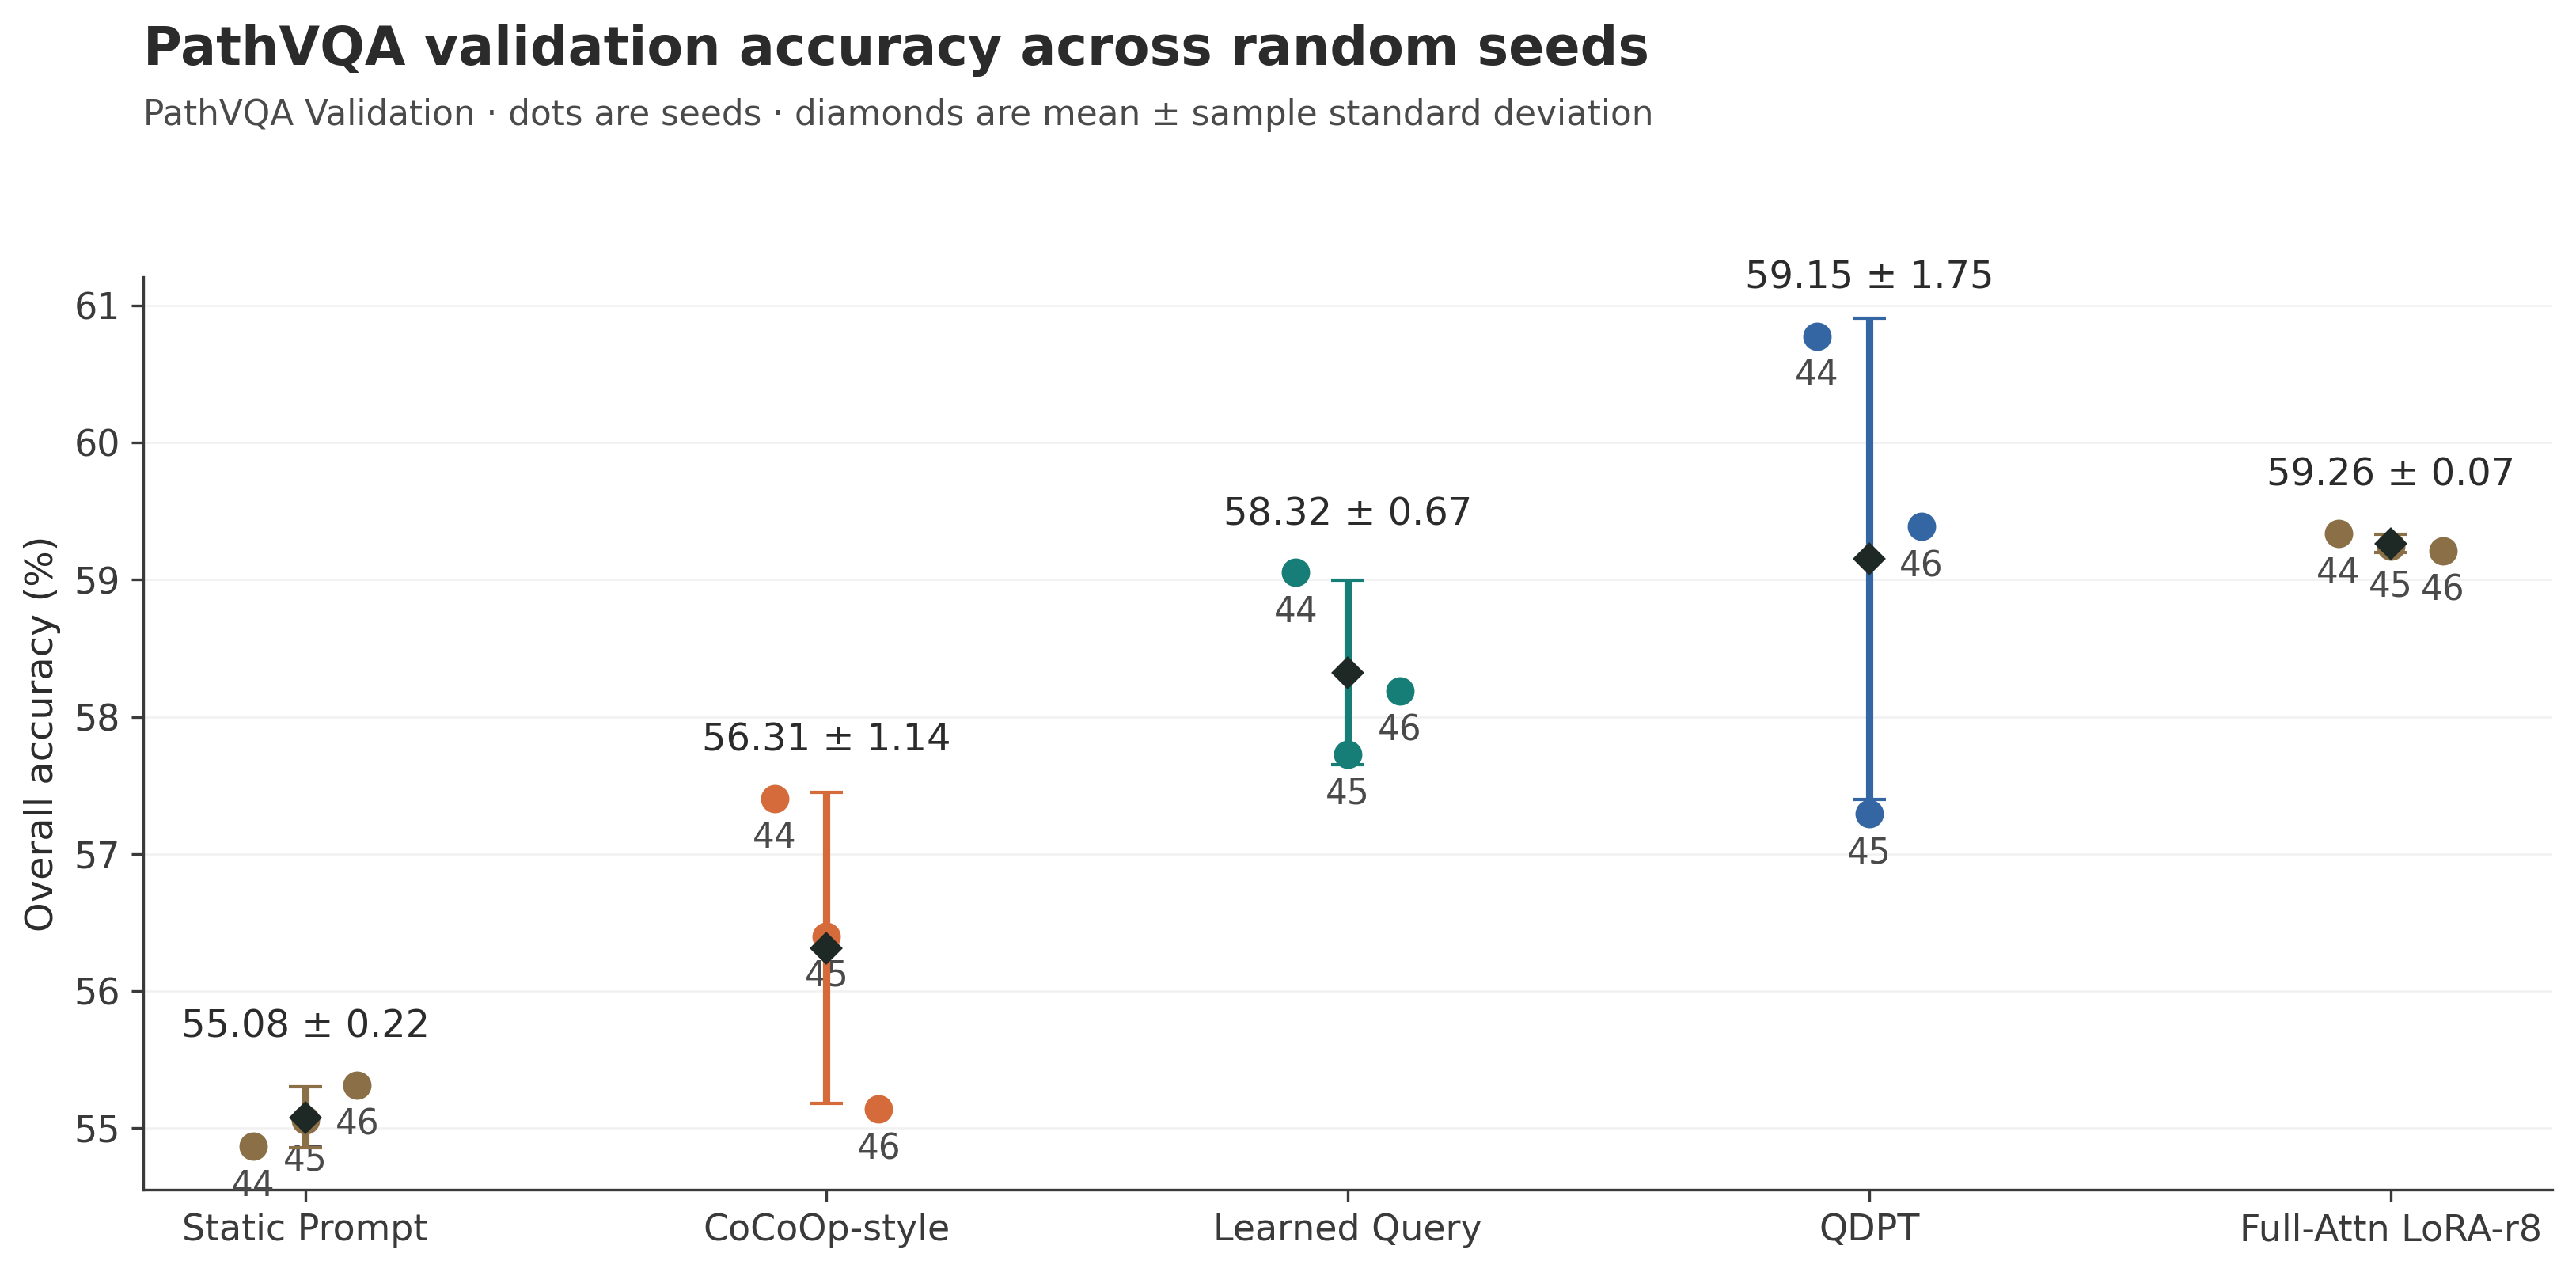
\includegraphics[width=\textwidth,trim=0 0 0 42bp,clip]{figures/pathvqa_seed_stability.png}
    \caption{PathVQA Validation Overall的三随机种子分布。圆点表示单次运行，菱形和误差线表示均值与样本标准差。}
    \label{fig:seed-stability}
\end{figure}

\subsection{结果讨论}

QDPT在PathVQA Validation上与LoRA取得接近的平均准确率，在SLAKE上则落后4.87个百分点。电气实验中，QDPT比LoRA多答对4题，这组单次结果用于设备图像上的应用验证。SLAKE的分项差距更有解释价值：QDPT在KVQA和OPEN上分别落后8.24和6.12个百分点，说明当前Prompt接口对知识型问题和开放回答的适配仍然不足。

机制消融分别检验问题条件化和视觉读取。采用$\mathcal{S}_{f}$时，问题条件Query的三次运行均值比可训练参数量相同的Learned Query高0.83个百分点，但seed 45出现反转。采用$\mathcal{S}_{o}$时，关闭动态分支的视觉读取使准确率由59.56\%降至57.63\%，移除静态视觉Prompt后为58.44\%。后两项的配对检验和图像聚类Bootstrap支持观察到的单次运行差值。

位置实验呈现出另一种现象。seed 44支持当前排列，seed 45却出现反转，三种排列的均值差也明显小于QDPT自身的运行波动。位置会影响训练轨迹，但优势方向依赖初始化。因此，当前输入顺序应视为Validation阶段固定下来的实现选择，不承担核心机制证据。

QDPT有7.805M可训练参数，约占4.445B骨干的0.18\%，略多于LoRA的7.078M。在统一微批量、样本序列和视觉Token数量的短程测试中，QDPT的训练吞吐为LoRA的1.88倍，峰值分配显存低18.18\%。这项差异来自当前两种适配实现的完整训练路径，尚未拆分到具体算子。附录中的输出头压缩减少了参数量，却带来3.36个百分点的准确率损失，没有改善本次实验的精度与容量折中。

训练稳定性仍是QDPT的不足。PathVQA上，QDPT三次运行的标准差为1.75，高于静态Prompt的0.22和CoCoOp-style的1.14。Test上的Free-form标准差为2.49，也高于Yes/No的1.15。较大的运行间差异可能与动态生成器的联合优化有关，现有诊断尚未定位主要来源。问题池化对固定Token集合的排列不敏感，也限制了动态分支对词序关系的表达。后续可分别考察问题编码方式和生成器优化设置，以改善关系表达与训练稳定性。
